\chapter{Introduction}
\label{ch:introduction}

\section{On Artificial Intelligence (AI) and Computational Linguistics}
% copied from intro
In 1950 Alan Turing in a seminal paper \citep{Turing1950} published in Mind was asking if ``machines can do what we (as thinking entities) can do?'' He questioned what intelligence was and whether it could be manifested in machine actions indistinguishable from human actions. 

He proposed the famous \textit{Imitation Game} also known as the \textit{Turing test} in which a machine would have to exhibit intelligent behaviour equivalent or indistinguishable from that of a human. The test was set up by stating the following rules. The machine (player A) and a human (player B) are engaged in a written \textit{natural language} conversation with a human judge (player C) who has to decide whether each conversation partner is human or a machine. The goal of players A and B is to convince the judge (player C) that they are human. 

This game underpins the question whether ``a computer, communicating over a teleprinter, (can) fool a person into believing it is human?'', moreover, whether it can exhibit (or even appear to exhibit) human(-like) cognitive capacities \citep{Harnad1992}. Essential parts of such cognitive capacities and intelligent behaviour that the machine needs to exhibit are of course the linguistic competences of comprehension (or ``understanding'') and generation of ``appropriate'' responses (for a given input from the judge C).

The \textit{Artificial Intelligence} (AI) field was born from dwelling on Turing's questions. The term was coined by McCarthy for the first time in 1955 referring to the ``science and engineering of making intelligent machines'' \citep{McCarthy1955}.

The general target is to program machines to do with language what humans do. Various fields of research contribute to this goal. Linguistics, amongst others, contributes with theoretical frameworks systematizing and accounting for language in terms of morphology, phonology, syntax, semantics, discourse or grammar in general. In computer science increasingly more efficient algorithms and machine learning techniques are developed. Computational linguistics provides methods of encoding linguistically motivated tasks in terms of formal data structures and computational goals. In addition, specific algorithms and heuristics operating within reasonable amounts of time with satisfiable levels of accuracy are tailored to accomplish those linguistically motivated tasks.

\textit{Computational Linguistics} (CL) was mentioned in the 1950 in the context of automatic translation \citep{Hutchins1999} of Russian text into English and developing before the field of Artificial Intelligence proper. Only a few years later CL became a sub-domain of AI as an interdisciplinary field dedicated to developing algorithms and computer software for intelligent processing of text (leaving the very hard questions of intelligence and human cognition aside). Besides \textit{machine translation} CL incorporates a broader range of tasks such as \textit{speech synthesis and recognition, text tagging, syntactic and semantic parsing, text generation, document summarisation, information extraction} and others. 
%New higher level and more complex tasks are formulated in academic and business environments as the simpler ones receive satisfiable 

This thesis contributes to the field of CL and more specifically it is an advancement in \textit{Natural Language Parsing} (NLP), one of the central CL tasks informally defined as the process of transforming a sentence into (rich) machine readable syntactic and semantic structure(s). Developing a program to automatically analyse text in terms of such structures by involving computer science and artificial intelligence techniques is a task that has been pursued for several decades and still continues to be a major challenge today. This is especially so when the target is \textit{broad language coverage} and even more when the desired analysis goes beyond simple syntactic structures and towards richer functional and/or semantic descriptions useful in the latter stages of \textit{Natural Language Understanding} (NLU). The current contribution aims at a reliable modular method for parsing unrestricted English text into a feature rich constituency structure using Systemic Functional Grammars (SFGs). 

In computational linguistics, broad coverage natural language components now exist for several levels of linguistic abstraction, ranging from tagging and stemming, through syntactic analyses to semantic specifications. In general, the higher the degree of abstraction, the less accurate the coverage becomes and, the richer the linguistic description, the slower the parsing process is performed. 

Such working components are already widely used to enable humans to explore and exploit large quantities of textual data for purposes that vary from the most theoretical, such as understanding how language works or the relation between form and meaning, to very pragmatic purposes such as developing systems with natural language interfaces, machine translation, document summarising, information extraction and question answering systems to name just a few. 

%end copied from intro

\section{Living in technologically ubiquitous world}
\label{sec:motivation}
Developed over thousands of years, the human language has become a versatile highly nuanced form of communication that carries a wealth of meaning which by far transcends the words alone. When it comes to \textit{human-machine} interaction this highly articulated communication form is deemed impractical. So far humans had to learn to interact with computers and do it in  formal, strict and rigorous manner via graphical user interfaces, command line terminals and programming languages. Advancements in \textit{Natural Language Processing} (NLP) which is a branch of \textit{Artificial Intelligence} (AI) are a game changer in this domain. NLP starts to unlocks the information treasure locked in the human speech and make it available for processing to computers. NLP becomes an important technology in bridging the gap between natural data and digital structured data.

In a world such ours, where technology is ubiquitous and pervasive in almost all aspects of our life, NLP becomes of great value and importance regardless whether it materializes as a spell-checker, intuitive recommender system, spam filter, (not so) clever machine translator, voice controlled car, intelligent assistants such as Siri, Alexa or Google Now. 

Every time you ask Siri or Alexa for directions to the nearest Peruvian restaurant, how to cook Romanian beef stew or what is the dictionary definition for the word ``germane'', a complex chain of operations is activated that allows `her' to understand the question, search for the information you are looking for and respond in a human understandable language. Such tasks are possible only in the past few years thanks to advances in NLP. Until now we have been interacting with computers in a language they understand rather than us. Now they are learning our language. 

%\section{NLP for business}
%\label{sec:motivation-business}

NLP opens new and quite dramatic horizons for businesses. Navigating with limited resources stormy markets of competitors, customers and regulators and finding an optimal answer/action to a business question is not a trivial task. 
Markets are influenced by the information exchange and being able to process massive amounts of text and extract meaning can help asses the status of an industry and play an essential role in crafting a strategy or a tactical action. 
Relevant NLP tasks for gathering market intelligence are \textit{named entity recognition} (NER), \textit{event extraction} and \textit{sentence classification}. With these tasks alone one can build a database about companies, people, governments, places, events together with positive or negative statements about them and run versatile analytics to audit the state of affairs.

Compliance with governmental, European or international regulations is a big issue for large corporations. One question for addressing this problem is whether a product is a liability or not and if yes then in which way. Pharma companies for example, once a drug has been released for clinical trials, need to process the unstructured clinical narratives or patient's reports about their health and gather information on the side effects. The NLP tasks needed for this applications are primarily \textit{NER} to extract names of drugs, patients and pharma companies and \textit{relation detection} used to identify the context in which the side effect is mentioned. NER task help transforming a sentence such as ``Valium makes me sleepy'' to ``(drug) makes me (symptom)'' and relation detection will apply patterns such as ``I felt (symptom) after taking (drug)'' to detect the presence of side effects.

Many customers, before buying a product, check online reviews about the company and the product whether it is pizza or a smartphone. Popular sources for such inquiry are the blogs, forums, reviews, social media, reports, news, company websites, etc. All of them contain a plethora of precious information that stays trapped in unstructured human generated text. This information if unlocked can play a great deal in company's reputation management and decisions for necessary actions to improve it. The NLP tasks sufficient to address this business required are \textit{sentiment analysis} to identify attitude, judgement, emotions and intent of the speaker, and \textit{co-reference resolution} which connects mentions of things to their pronominal reference in the following or preceding text. These tasks alone can extract the positive and negative attitudes from sentence ``The pizza was amazing but the waiter was awful!'' and connect it to the following sentence ``I adore when it is topped with my favourite artichoke'' about pizza and not the waiter and discover a topping preference.

NLP is heavily used in customer service in order to figure out what customer means not just what she says. Interaction of companies with their customers contain many hints pointing towards their dissatisfaction and interaction itself is often one of the causes. Companies record, transcribe and analyse large numbers of call recordings for extended insights. They deploy chat bots fo increased responsiveness by providing immediate answers to simple needs and also decrease the load of the help desk staff. NLP tasks that are essential in addressing some of the customer service needs are \textit{speech recognition} that converts speech audio signal into text and \textit{question answering} which is a complex task of recognising the human language question, extract the meaning, searching relevant information in a knowledge base and generate an ineligible answer. Advances in deep learning allow nowadays to skip the need for searching in a knowledge base by learning from large corpora of question-answer pairs complex interrelations. 

The above cases underline the increased need in NLP whereas the variation and ever increasing complexity of tasks reveal the need in deeper and richer semantic and pragmatic analysis across a broad range of domains and applications. Any analysis of text beyond the formal aspects such as morphology, lexis and syntax inevitably lead to a functional paradigm of some sort which can be applied not only at the clause level but at the discourse as a whole. This makes the text also an artefact with relation socio-cultural context where it occurs. 

\section{The linguistic framework}
\label{sec:framework}
Any description or analysis involving language implies some theory of about its essential nature and how it works. A linguistic theory includes also goals of linguistics, assumptions about which methods are appropriate to approach those goals and assumptions about the relation between theory, description and applications \citep[3]{Fawcett2000}. 

In his seminal paper ``Categories of the theory of grammar'' \citep{Halliday61-orig}, Halliday lays the foundations of \textit{Systemic Functional Linguistic} (SFL) following the works of his British teacher J. R. Firth, inspired by Louis Hjelmslev \citep{Hjelmslev53} from Copenhagen School of linguistics and by a group of European linguists from Prague Linguistic Circle. This paper constitutes a response to the need for a \textit{general theory of language} that would be holistic enough to guide empirical research in the broad discipline of linguistic science:
\begin{quotation}
    \dots the need for a \textit{general} theory of description, as opposed to a \textit{universal} scheme of descriptive categories, has long been apparent, if often unformulated, in the description of all languages \citep[54; emphasis in original]{Halliday57}
    \dots
    If we consider general linguistics to be the body of theory, which guides and controls the procedures of the various branches of linguistic science, then any linguistic study, historical or descriptive, particular or comparative, draws on and contributes to the principles of general linguistics \citep[55]{Halliday57}
\end{quotation} 

% deeper on SFL

%TODO: use here metrial from Bateman2017-sfl [the place of systemic functional linguistics ... 21 century]

SFL regards language as a social semiotic system where any act of communication is regarded as a conflation of \textit{linguistic choices} available in a particular language. Choices are organised on a paradigmatic rather than structural axis and represented as \textit{system networks}. Moreover, in the SFL perspective language has evolved to serve particular \textit{functions} influencing their the structure and organisation of the language. However, their organisation around the paradigmatic dimension leads to a significantly different functional organisation than those found in several other frameworks which \citet{Butler2003-pt1, Butler2003-pt2} addresses extensively. 
Also, making the paradigmatic organization of language a primary focus of linguistic description decreased the importance of the formal structural descriptions which from this perspective appear as realisation of (abstract) features. 

Embracing the \textit{oragnon model} formulated by \citet{Buhler34}, Halliday refers to the language functions as metafunctions or lines of meaning that offer a trinocular perspective on language through \textit{ideational}, \textit{interpersonal} and \textit{textual} metafunctions. In SFL, language is first of all an interactive action serving to enact social relations under the umbrella of the \textit{interpersonal metafunction}. Then it is a medium to express the embodied human experience of inner (mental) and outer (perceived material) worlds via \textit{ideational metafunction}. Finally the two weave together into a coherent discourse flow whose mechanisms are characterised through the \textit{textual metafunction}. 

Then a linguistic description is provided at various levels of granularity, that in SFL are is called \textit{delicacy}. Just like the resolution of a digital photo defines the clarity and the amount of detail in the picture, the same way delicacy refers to the how fine- or coarse-grained distinctions are made in the description of the language. And if other linguistic traditions speak of a \textit{grammar} in SFL the term \textit{lexico-grammar} is used which, intuitively, is the combination of grammar and lexis explained in Section \ref{sec:wording} into a unitary body. A deeper description of the SFL theory of language is provided latter in Chapter \ref{ch:sfg}.

% on metafunctions
%TODO briefly introduce and refere to other extensive sources
%To account for the complexity and phenomenological diversity of human language the SFL theory provides descriptions along \textit{syntagmatic, (meta)functional, paradigmatic, stratification and instantiation axes}. 

% 
Until today, two major Systemic Functional Grammars (SFG) have been developed: the \textit{Sydney Grammar} \citep{Halliday2013} and the \textit{Cardiff Grammar} \citep{Fawcett2008}. The latter, as Fawcett himself regards it, is an extension and a simplification of Sydney Grammar \citep[xviii]{Fawcett2008}. Each of the two grammars has advantages and shortcomings (presented in Chapter \ref{ch:sfg}) which I discuss from the perspective of theoretical soundness and suitability to the goals of the current project.

Both Cardiff and Sydney grammars had been used as language models in natural language generation projects within 
the broader contexts of social interaction. Some researchers \citep{Kasper1988, ODonoghue1991a, ODonnell1993, Souter1996, Day2007} attempted to reuse the grammars for the purpose of syntactic parsing within the borders of NL generation coverage. I come back to these works in more detail in Section \ref{sec:sota}.

% in short

To sum up, in this thesis I adopt the Systemic Functional Linguistic (SFL) framework because of its versatility to account for the complexity and phenomenological diversity of human language providing descriptions along \textit{multiple semiotic dimensions} i.e. paradigmatic, syntagmatic, meta-functional, stratification and instantiation dimensions \citep{Halliday2003} and at different \textit{delicacy levels} of the \textit{lexico-grammatical cline} \citep{Halliday2002, Hasan2014}.  These notions and other elements of the SFL theory are addressed below in Chapter \ref{ch:sfg}.

%todo motivational introduction for other kinds of applications of SFL
%As we part away from the surface form of text and aim for rich semantics or aim at analyses higher than the clause level i.e. discourse, the functional is increasingly useful and revealing of meanings in text. Such analyses have been done manually by linguists, semioticians and educators in an informal manner as there have not been any tools to automate such processes. Besides Linguistics, there is a plethora of linguistic analysis using SFL framework in other fields of research. SFL has been used extensively as a descriptive framework in Critical Discourse Analysis and in Education studies. Automatising the language analysis with SFL framework will unlock the potential of these fields. Next I provide a glimpse of what opportunities they offer. 

\section{An example of Systemic Functional analysis}
\label{sec:example}
To provide a better intuition, this section describes an analysis of sentence using SFL framework. Here a parallel analysis between SFL and a more traditional grammar is provided in order to highlight the richness and high descriptive potential of SFL grammars. A source of the descriptive abundance is achieved through a practice of feature systematisation as mutually exclusive choices which is exemplified as well for three features of traditional grammar below. The feature analysis provided here is partial and restricted to only two constituents as this suffices to provide the reader with an intuition of what to expect from an SFL analysis.

Traditional linguistics teaches us how to carry on a syntactic analysis of a sentence. So let's consider Example \ref{ex:1} in order to perform one. First we would assign a \textit{part of speech} (verb, noun, adjective etc.) to each word, then we would focus on clustering words into constituents guided by the intuitive rule \textit{which words goes together}, and then those would receive syntactic functions (subject, predicate, complement etc.) within the sentence.   %and result in a grouping such as the one in Example \ref{ex:2}. 

\begin{exe}
    \ex\label{ex:1} He gave the cake away.
%    \ex\label{ex:2} He gave (the cake) away .
\end{exe}

\begin{figure}[!ht]
    \centering
    \begin{tikzpicture}[tree-style,level 1/.style={sibling distance=4em},
    level 2/.style={sibling distance=4em}, level distance=4.5em]
    \node (cla) [pattern-node] {\textit{He gave the cake away.}}
    child { node (sub)[pattern-node] {He}}		
    child { node (mv)[pattern-node] {gave}}
    child { node (com)[pattern-node] {\textit{the cake}}
        child { node (det)[pattern-node]{the}}
        child { node (nou)[pattern-node]{cake}}}
    child {node[pattern-node](adjunct)
        {away}
    };
    \end{tikzpicture}
    \caption{Representation of the Example \ref{ex:1} as constituency tree}
    \label{fig:mcg-graph-example-simple-structure}
\end{figure}

Figure \ref{fig:mcg-graph-example-simple-structure} depicts the constituency division of the clause \ref{ex:1}% which is identical to the bracket notation in Example \ref{ex:2}. 
The nodes represent grammatical constituents and the edges stand for the \textit{structure-substructure composition}. 
Next we can move on to assign constituent class and a grammatical function. Table \ref{tab:sfg-constituency-analisys} provides a constituency analysis in SFL tradition. Here the sentence is formed of a single clause which has four constituting functional parts: a Subject, a Main Verb (also known as Predicate), a Complement and an Adjunct. Each of these functional parts is filled correspondingly by a pronoun, a verb, a nominal group and an adverb as assigned in the table below.

\begin{table}[!ht]
    \centering
    \begin{tabular}{cc|c|c|c}
        \hline
        \multicolumn{1}{|c|}{\textit{He}} & \textit{gave} & \textit{the}     & \textit{cake}   & \multicolumn{1}{c|}{\textit{away.}} \\ \hline
        \multicolumn{5}{|c|}{clause}                                                                                                 \\ \hline
        \multicolumn{1}{|c|}{Subject}     & Main Verb     & \multicolumn{2}{c|}{Complement}    & \multicolumn{1}{c|}{Adjunct}        \\ \hline
        \multicolumn{1}{|c|}{pronoun}      & verb          & \multicolumn{2}{c|}{nominal group} & \multicolumn{1}{c|}{adverb}         \\ \hline
        &               & Deictic          & Thing           &                                     \\ \cline{3-4}
        &               & determiner       & noun            &                                     \\ \cline{3-4}
    \end{tabular}
    \caption{Constituency analysis with unit classes and grammatical functions (table view)}
    \label{tab:sfg-constituency-analisys}
\end{table}

Next each constituent can be assigned a set of relevant linguistic features. For example The subject ``He'' is a pronoun that has features known in traditional grammar: \textit{singular}, \textit{masculine}, and \textit{3^{rd} person}. These features are well differentiated in traditional grammar. For example \textit{singular} means \textit{non-plural}, \textit{masculine} means \textit{non-feminine} and \textit{3^{rd} person} means \textit{non-1^{st}} and \textit{non-2^{nd}}. These are closed classes meaning that there is no \textit{4^{th} person} or that there is no \textit{neutral} grammatical gender in English as other languages have. These features can be systematised (see Figure \ref{fig:traditional-pronoun}) as three systems of mutually exclusive choices that can be assigned to pronominal units. Note that the gender is enabled for 3^{rd} person singular pronouns which can be expressed as is the figure below representing a \textit{system network} (explained in Chapter \ref{ch:sfg}).

\begin{figure}[!ht]
    \centering      
    \includegraphics[width=.56\textwidth]{Figures/Example/traditional-pronoun.pdf}      
    \caption{The systematisation of three pronominal features in traditional grammar}
    \label{fig:traditional-pronoun}
\end{figure}

In SFG the pronouns are systematised in the system network of Person from \textit{Introduction to Functional Grammar} \citep[366]{Halliday2013} that is depicted in Figure \ref{fig:person-system-network}. The red rectangles from the figure represent the selections that are applicable to the Subject constituent ``He'' in example above.

\begin{figure}[!ht]
    \centering      
    \includegraphics[width=.90\textwidth]{Figures/Example/person-selections.pdf}      
    \caption{The selections in Person system network from \citet[366]{Halliday2013} }
    \label{fig:person-system-network}
\end{figure}

Lets take now the clause constituent that is the root of the constituency tree and see how SFL features can be applied to it. If in in terms of traditional grammar the clause can be ascribed relatively few features i.e. as having \textit{passive voice}, \textit{positive polarity} and \textit{simple past tense} then in terms of SFL grammar the features are many more i.e. \textit{major, positive, active, effective, receptive, agentive, free, finite, temporal, past, non-progressive, non-perfect, declarative, indicative, mood-non-assessed, comment-non-assessed}. Figure \ref{fig:mood-selections} depicts the selections applicable to clause constituent in Example \ref{ex:1} from Mood system network that is an adaptation of Mood network proposed in \citet[162]{Halliday2013}. 

\begin{figure}[!ht]
    \centering      
    \includegraphics[width=0.91\textwidth]{Figures/Example/mood-selections.pdf}      
    \caption{The feature selections in the Mood system network for Example \ref{ex:1}}
    \label{fig:mood-selections}
\end{figure}

So far you have seen constituents assigned syntactic functions such as Subject, Complement, Adjunct etc. SFL covers a wider range of functions depending on the kind of meaning it aims at describing. For example what in other grammars is known as \textit{semantic labels}, \textit{thematic} or \textit{$\theta$ roles} SFL systematises as Transitivity system network (which will be introduced in Chapter \ref{sfg} below). Transitivity aims at providing domain independent \textit{semantic frames} called in SFL \textit{process configurations} which describe semantic actions and relationships, along with \textit{semantic roles} ascribed to their \textit{participants}. These semantic frames generally are governed by verbs and more specifically each verb meaning has a dedicated semantic frame. 

For example \ref{ex:1} corresponds to a Possessive semantic frame where ``He'' is the Agent and Carrier whereas ``the cake'' is the Possessed thing as marked in Example \ref{ex:3}. These configurations and participant roles correspond to Transitivity system network proposed in \citep{Neale2002}.

\begin{exe}
    \ex\label{ex:3} [_{Agent-Carrier} He] gave [_{Possessed} the cake] away. 
\end{exe}

There are more functions and features that can be assigned to the constituents in the Example \ref{ex:1} but I stop here. The analysis provided so far highlights that SFG grammar has a variety of functions serving to express different meanings. The traditional grammar distinguishes them as syntactic and semantic functions but, as we will see in Chapter \ref{ch:sfg} below, SFL does not make such a distinction. Another aim of the current section was to provide a glance of the feature rich grammar and I hope the example with Mood feature selection in Figure \ref{fig:mood-selections} fulfils this goal.

\begin{figure}[!ht]
    \centering
    \begin{tikzpicture}[scale=0.8, transform shape, tree-style, 
    level 1/.style={sibling distance=11em, level distance=14em},
    level 2/.style={sibling distance=10em, level distance=12em}, 
    anchor=north
    growth parent anchor = north,]
    
    \node (cla) [pattern-node, split-node, text width = 42em,]  
    {clause 
        \nodepart{two} Configuration
        \nodepart{three} major, positive, active, effective, receptive, agentive, free, finite, temporal, past, non-progressive, non-perfect, declarative, indicative, mood-non-assessed, comment-non-assessed, posessive};
    
    \node (sub) [pattern-node, split-node, below=3em of cla, xshift=-16em,] 
    {pronoun
        \nodepart{two} Subject, Participant,\\ 
        Agent \& Carrier 
        \nodepart{three} 3^{rd} person, singular,\\ 
        male, non-interactant,\\ 
        one-referent, conscious};
    
    \node (mv)[pattern-node, split-node, below=3em of cla, xshift=-5em] 
    {verb
        \nodepart{two} Main Verb, Finite, \\Process 
        \nodepart{three} possessive };
    
    \node (com)[pattern-node,split-node, below=3em of cla, xshift=6em] 
    {nominal group
        \nodepart{two} Complement, Participant, 
        \\ Affected \& Possessed
        \nodepart{three} };
    
    \node (det)[pattern-node,split-node, below=3em of com, xshift=-6em]
    {determiner
        \nodepart{two} Deictic, Modifier
        \nodepart{three} specific, demonstrative,\\ 
        determinative, non-selective};
    
    \node (nou)[pattern-node,split-node, below=3em of com, xshift=6em]
    {noun
        \nodepart{two} Thing, Head
        \nodepart{three} inanimate, singular,\\ 
        countable };
    
    \node[pattern-node,split-node, below=3em of cla, xshift=17em](adjunct)
    {adverb
        \nodepart{two} Adjunct,
        \\Circumstance,
        \\Location
        \nodepart{three} };
    
    \draw[sequence,-,edge-style] (cla.south) -- ++(0,-1em) -| (sub.north);
    \draw[sequence,-,edge-style] (cla.south) -- ++(0,-1em) -| (mv.north);
    \draw[sequence,-,edge-style] (cla.south) -- ++(0,-1em) -| (com.north);
    \draw[sequence,-,edge-style] (cla.south) -- ++(0,-1em) -| (adjunct.north);
    \draw[sequence,-,edge-style] (com.south) -- ++(0,-1em) -| (det.north);
    \draw[sequence,-,edge-style] (com.south) -- ++(0,-1em) -| (nou.north);	
    \end{tikzpicture}
    \caption{Representation of Example \ref{ex:1} as feature rich constituency tree}
    \label{fig:mcg-graph-example}
\end{figure}


Next, Figure \ref{fig:mcg-graph-example} summarises everything discussed above into a partially filled constituency tree. The constituents that were not discussed are assigned only few high level functions and features. As you can see, every node is richly decorated with syntactic and semantic features. The blue part of each node denotes grammatical class, the red part carries functions some of  which are important to establishing a valid constituency structure (that are Mood functions) and the the Transitivity functions; and the green part some grammatical features selected from system networks. In practice, the feature set is much richer than what nodes in Figure \ref{fig:mcg-graph-example} carry here the restriction aims simply to avoid an over-crowded example. 


%Generating automatically feature rich constituency structure such as the one in Figure \ref{fig:mcg-graph-example} is the general aim in the current work.

Next I describe what opportunities and limitations exist in automatically generating rich SFL analyses as until now it has not been possible to use these detailed analysis in computational contexts. This makes them unavailable for corpus work, for training data in machine learning and other end-user application scenarios provided as motivation in the Sections \ref{sec:motivation} above.

\section{Computing with SFG - a practical problem}
\label{sec:problem}
%the problem of parsing with SFGs

%\todo[inline]{
%    But, until now it has not been possible to use these
%    detailed analysis in computational contexts: this makes
%    them unavailable for corpus work, for training data in
%    machine learning, etc. etc. (add as many points as occur
%    to you).
%}

%\todo[inline]{
%    There have been attempts to make this work (which you
%    will come back to and describe in Chapter X in detail), however,
%    but these have not worked. As you you say you will describe in detail
%    in Chapter X, }

%\todo[inline]{
%    there is however a strong diagnostic as to
%    just why these attempts have not been successful: i.e., the
%    lack of structural detail that SFG descriptions typically
%    provide. This is argued in general in Bateman (2008)
%    and Teich (1999) [and any other references you can find].
%}

%The problem of parsing with SFG has been well laid out in \citet{Bateman2008} as being one of computational complexity due to exponential explosion of possible combinations of features. 

SFL since it has been established has been primarily concerned with the paradigmatic axis of language. Accounts of the syntagmatic axis of language, for example syntactic structure, have been put in the background. The structure has been placed on the theoretical map and defined in terms of \textit{rank}, \textit{unit}, \textit{class} and \textit{function}, as we will see in detail in Chapter \ref{ch:sfg} but afterwards it received minimal attention as most of the focus was on the paradigmatic organisation in language (in fact this is is the feature that sets SFL apart from other approaches to study language). This has led to progress in accounting how language works at all strata but little was said about the language constituency. And this can be considered ``unsolved'' within SFL accounts leaving a ``gap in what must be one the central areas of any characterisation of language'' \citep[25]{Bateman2008}. 

%As we will see below, some accounts of constituency are provided within SFL grammars, enough even to make them applicable in computational domains such as automatic \textit{natural language generation}. But such descriptions are by far not satisfiable with respect to what would a proper syntagmatic account of language would be. 

This may be surprising as the syntagmatic dimension is implicit and present everywhere in the SFL literature. For instance all example analyses in the \textit{Introduction to Functional Grammar} \citep{Halliday2013} are predominantly syntagmatic. Moreover, Robin Fawcett for decades promotes the motto \textit{no system network without realisation statements} \citep[9]{Fawcett88-good}. \citet{Bateman2008} presents in detail why there is a severe imbalance between syntagmatic and paradigmatic axes in SFL, how it came to be this way and how it is especially damaging to the task of automatic text analysis. Next I describe the main problems and hint at how potential solutions may look like (described Section \ref{sec:solution}). 

\citet{ODonnell2005} offer a detailed description to the long history of SFL being applied in computational contexts yielding with productive outcomes on language theorising, description and processing. The transfer between SFL and computation typically involved a delay between the theoretical formulation and the computational instantiation of that formulation \citep[139]{BatemanMatthiessen88} \citep[19]{MatthiessenBateman91}. The theoretically formulated ideas contain hidden pitfalls that are revealed only upon explicit formulations required by in computation \mbox{\citep[27]{Bateman2008}}. 

The active exchange between the SFL theory and computation has been almost entirely oriented towards automatic \textit{natural language generation}. Such systems would use abstract semantic specifications and communicative goals to produce grammatically correct and well connected texts achieving those goals. This area has been shown to be successful in part due to decomposition of language along the paradigmatic axis using functionally motivated sets of choices between functionally motivated alternatives \citep{McDonald80}.

The computational processes driving the natural language generation relied heavily on the notion of \textit{search}. A well defined search problem is defined in terms of a precise description of the search space which then helps navigation process effectively to find solutions. The paradigmatic organization of the \textit{lexicogrammar} as system networks assumed within SFL turns out to organise the search space for possible grammatical units appropriate for communicative goals in almost ideal manner \citep[28]{Bateman2008}.

The \textit{automatic analysis} or \textit{parsing} can be seen as a reverse problem of finding appropriate analysis within a search space of possible solutions. That is identify the exact meaning, systematised in the grammar, of a given natural language sentence. As seen in Section \ref{sec:example} above, an account of the sentence meaning would have to provide both, in terms of a formal structure of the sentence revealing the constituents plus their syntactic relations to each other, and in terms of a complete set of features (detailed to the extent that grammar permits) applicable to each constituent of structure. If, in the generation process, the abstract semantic specifications are increasingly materialised through choice making by traversing the system network towards finally generated text, then, in the parsing process, the reverse is the case. The process starts from a given sentence aiming to derive/search the feature choices in the system network afferent to each of the constituents. But if the paradigmatically organised lexicogrammatical resource is effective for generation it turns out, as we will see next, to be by far unsuitable for the analysis task because of the \textit{size problem}. Halliday himself mentions this problem when he asks \textit{how big is a grammar?}.

\begin{quotation}
    Given any system network it should in principle be possible to count the number of alternatives shown to be available. In practice, it is quite difficult to calculate the number of different selection expressions that are generated by a network of any considerable complexity \citep[10]{Halliday96-grammatics}.
\end{quotation}

The issue emerges from the way connections and (cross-)classifications are organised in a system network. In addition to that, the orientation of systemic grammars towards choice means that the grammar full of disjunctions leading to the problem of search complexity. Also the abstract nature of systemic features leads to a structural richness that adds logical complexity to the task \citep{ODonnell1993}. So estimating the size of the grammar would in fact mean estimating the potential number of feature combinations. For example, a hypothetical network of 40 systems the ``size of the grammar it generates lies somewhere between 41 and 2^{40} (which is somewhere around 10^{12})'' \citep[28]{Bateman2008}. However it is not easy to predict where would the upper limit of the grammar would fall even when the configuration of relations of a particular system network is known.

For the generation task, that size, is not a problem at all as the number of choice points is actually rather small. Such a paradigmatic organisation is, in fact, an incredibly concise and efficient way to express the linguistic choices where the possible feature selections are relevant only when they are enabled by prior paradigmatic choices and it is only those alternatives that need to be considered \citep[12--13]{Halliday96-grammatics} .

In the analysis task, the paradigmatic context of choice, that helps navigation during the generation process, is no longer available. It is not known
any longer which features of a systemic network are relevant and which are not. This leads to a radical asymmetry between the two tasks. That
is: in generation, the simple traversal of the network finds only the compatible choices
because that is what the network leads to; whereas in analysis it is not evident in
advance which path to follow therefore the task is virtually to explore entire search
space in order to discover which features apply to the text. This means that any path is potentially relevant and shall be passed and checked leading to evaluation of the system network as a whole; and that there is no way to restricting the search space, as in the case of generation, to a a set of familiar paradigmatic lines \citep[29]{Bateman2008}. 

One of the grammars successfully used in generation tasks is Nigel grammar developed within Penman generation project \citep{Mann83}. It contains 767 grammatical systems defined over 1381 grammatical features which Bateman evaluates as ``a very large computational grammar by current standards, although nowadays by no means the broadest when considered in terms of raw grammatical coverage'' \citep[29]{Bateman2008}. To parse with such a grammar would means exploring an incredibly vast search space $ 3 \times 10^{18} $ to be more precise. A more detailed break down the complexity by rank or primary class as provided in Table \ref{tab:size} below.

\begin{table}[!ht]
    \centering
    \begin{tabular}{|l|r|}
        \hline
        \textit{rank or primary class} & \textit{size}                             \\ \hline
        adverbial-group                & 18                                        \\ \hline
        words                          & 253                                       \\ \hline
        quantity-group                 & 356                                       \\ \hline
        prepositional-phrase           & 744                                       \\ \hline
        adjectival-group               & 1045                                      \\ \hline
        nominal-group                  & \textgreater $ 2\times 10^{9} $  \\ \hline
        clause                         & \textgreater $ 3\times 10^{18} $ \\ \hline
    \end{tabular}
    \caption{Size of major components of the Nigel grammar expressed in terms of the number of selection expressions generated \citep[35]{Bateman2008}}
    \label{tab:size}
\end{table}

%difficulty SLR
Another difficulty in parsing with SFGs lays in the fact that, as the analysis moves away from directly observable grammatical variations towards more abstract semantic variations, the difficulty of generating an accurate account increases drastically. Transitivity system network for example consists of such semantic features and it is comparable to what is called in computational linguistics (shallow) \textit{semantic parsing} or \textit{Semantic Role Labelling} (SRL) \citep{Carreras2005}.

The main challenge of SRL (well explained in \citep[245--250]{gildea2002automatic}) remain the same since \citet{Winograd1972}: moving away from the domain specific, hand-crafted semantic specifications towards domain independent and robust set of semantic specifications. This goal was undertaken in several projects to build large broad-scope lexico-semantic databases such as WordNet \citep{Fellbaum98-wn}, FrameNet \citep{Baker1998, Johnson2000, fillmore2003background} and VerbNet \citep{schuler2005verbnet, Kipper2008}. A similar database exists for Transitivity system network as described in \citet{Fawcett2009} called Process Type Database \citep{Neale2002}. 

Such databases describe domain independent \textit{semantic frames} \citep{Fillmore1985} (know in SFL as \textit{configurations} or \textit{figures}) which describe semantic actions and relationships, along with \textit{semantic roles} ascribed to their \textit{participants}. The semantic frames generally are governed by verbs and more specifically each verb meaning has a dedicated semantic frame. For instance the perception frame contains \textit{Perceiver} and \textit{Phenomenon} roles as can be seen in Example \ref{ex:glance1}. 

\begin{exe}
    \ex\label{ex:glance1} [_{Agent-Perceiver} Jaqueline] glanced [_{Phenomenon} at her new watch].
\end{exe}

The tendency is to identify frames that are generic enough to cover classes of verb meanings (for example Action, Cognition, Perception, Possession frames) and the same applies to participant roles where the tendency is to reuse roles across semantic frames (for example agent role from Action frame is reused in Perception or Possession frames, or Phenomenon is reused in Cognition and Perception frames).

%example of covert constituents
Besides the challenge of pinning them down in text, the problem with semantic features goes one step further. Sometimes the semantic roles correspond to constituents that are displaced or not even realised in the text. This increases the challenge of identifying and assigning them correctly. Consider Example \ref{ex:glance2}. It is a sentence that has three non-auxiliary verbs: seem, worry and arrive. According to Cardiff grammar, which will be introduced in Chapter \ref{ch:sfg}, this corresponds to three clauses \textit{embedded} into each other as represented in Table \ref{tab:glance-analsys}.

\begin{exe}
    \ex\label{ex:glance2} She seemed to worry about missing the river boat.
%    \ex\label{ex:glance3} She seemed [to worry [about missing the river boat]].
\end{exe}

\begin{table}[!ht]
    \centering
    \resizebox{\columnwidth}{!}{%
    \begin{tabular}{cccc|c|c|c|c|c|}
        \hline
        \multicolumn{1}{|c|}{\textit{She}} & \multicolumn{1}{c|}{\textit{seemed}} & \multicolumn{1}{c|}{\textit{to}}        & \textit{worry} & \textit{about} & \textit{missing} & \textit{the} & \textit{river} & \textit{boat.} \\ \hline
        \multicolumn{9}{|c|}{clause}                                                                                                                                                                                              \\ \hline
        \multicolumn{1}{|c|}{Subject}      & \multicolumn{1}{c|}{Main Verb}       & \multicolumn{7}{c|}{Complement}                                                                                                               \\ \hline
        & \multicolumn{1}{c|}{}                & \multicolumn{7}{c|}{clause}                                                                                                                   \\ \cline{3-9} 
        & \multicolumn{1}{c|}{}                & \multicolumn{1}{c|}{Infinitive Element} & Main Verb      & \multicolumn{5}{c|}{Complement}                                                    \\ \cline{3-9} 
        &                                      &                                         &                & \multicolumn{5}{c|}{clause}                                                        \\ \cline{5-9} 
        &                                      &                                         &                & Binder         & Main Verb        & \multicolumn{3}{c|}{Complement}                \\ \cline{5-9} 
    \end{tabular}%
    }
    \caption{SF constituency analysis in Cardiff grammar style}
    \label{tab:glance-analsys}
\end{table}

The participant role configurations (or the semantic frames) these verbs bring about are provided in the Table \ref{tab:semantic-role-distro}. For the sake of this example lets say that the first role corresponds to the Subject constituent and the second to the Complement constituent. This way the verb meaning seem_{1} corresponds to an Attributive configuration that distributes Carrier and Attribute roles to the Subject ``She'' and the Complement ``to worry about missing the river boat''. In the case of worry about_1 and miss_1 the first roles provided by Cardiff grammar are \textit{compound} (i.e. composed of two simple ones) while the second ones are simple. So, in the example above, the verb meaning worry about_1 distributes the Phenomenon to the Complement ``about missing the river boat'' and the Agent \& Cognizant role to an empty Subject that is said to be \textit{non-realised}, \textit{covert} or \textit{null element}. A similar situation is for miss_1 that assigns an Affected \& Carrier role to the empty Subject and the Possessed role to the Complement ``the river boat''. 

\begin{table}[!ht]
    \centering
    \begin{tabular}{|l|l|l|}
        \hline
        \textit{verb meaning} & \textit{semantic configuration} & \textit{participant role mandatory distribution}  \\ \hline
        seem_{1}           & Attributive                     & Carrier + Attribute                     \\ \hline
        worry about_{1}   & Two Role Cognition              & Agent \& Cognizant + Phenomenon         \\ \hline
        miss_{1}           & Possessive                      & Affected \& Carrier + Possessed (thing) \\ \hline
    \end{tabular}
    \caption{Semantic role configurations according to \citet{Neale2002,Fawcett2009}}
    \label{tab:semantic-role-distro}
\end{table}

Those unrealised Subjects in the embedded clauses are recoverable from the immediate syntactic context (no need for discourse) and correspond, in this case, to the Subject in the higher clause. This is easy to see in Examples \ref{ex:glance3} and \ref{ex:glance4} therefore we can just mark the places of the null Subjects in the embedded clause in order to be able to assign the semantic labels (otherwise the frame cannot be assigned to the constituents). Notice that I have provided also an index \textit{i} to highlight that the null elements correspond to the higher clause Subject ``She''. 

\begin{exe}
    \ex\label{ex:glance3} \textit{She} worried about missing the river boat.
    \ex\label{ex:glance4} \textit{She} missed the river boat.
    \ex\label{ex:glance5} She_i seemed [\textit{null-Subject}_i to worry [about \textit{null-Subject}_i missing the river boat]].
\end{exe}

Now that the places of covert constituents are explicitly marked and the recoverable constituent coindexed we can see the distribution of semantic roles realised for this sentence in the Table \ref{tab:glance-analsys-semantic} below. 

\begin{table}[!ht]
    \centering
    \resizebox{\textwidth}{!}{%
        \begin{tabular}{cccccc|c|c|c|c|c|}
            \hline
            \multicolumn{1}{|c|}{\textit{She_i}}   & \multicolumn{1}{c|}{\textit{seemed}} & \multicolumn{1}{c|}{$\emptyset_i$}   & \multicolumn{1}{c|}{\textit{to}} & \multicolumn{1}{c|}{\textit{worry}} & \textit{about} & $\emptyset_i$ & \textit{missing} & \textit{the} & \textit{river} & \textit{boat.} \\ \hline
            \multicolumn{11}{|c|}{Attributive configuration}                                                                                                                                                                                                                         \\ \hline
            \multicolumn{1}{|c|}{Agent} & \multicolumn{1}{c|}{}       & \multicolumn{9}{c|}{Attribute}                                                                                                                                                                               \\ \cline{1-1} \cline{3-11} 
            & \multicolumn{1}{c|}{}       & \multicolumn{9}{c|}{Two Role Cognition configuration}                                                                                                                                                        \\ \cline{3-11} 
            & \multicolumn{1}{c|}{}       & \multicolumn{1}{c|}{Agent \& Cognizant} &                         & \multicolumn{1}{c|}{}               & \multicolumn{6}{c|}{Phenomenon}                                                                       \\ \cline{3-3} \cline{6-11} 
            &                             &                                      &                         & \multicolumn{1}{c|}{}               & \multicolumn{6}{c|}{Possessive configuration}                                                         \\ \cline{6-11} 
            &                             &                                      &                         &                                     &                & Affected \& Carrier &                  & \multicolumn{3}{c|}{Possessed}                 \\ \cline{7-7} \cline{9-11} 
        \end{tabular}%
    }
    \caption{Transitivity analysis in Cardiff grammar style \citep{Neale2002,Fawcett2009}}
    \label{tab:glance-analsys-semantic}
\end{table}

In language there are many cases where constituents are empty but recoverable from the immediate vicinity relying in most cases on syntactic means and in a few cases additional lexical-semantic resources are required. The mechanisms of detecting and resolving the empty constituents are captured in the Government and Binding Theory (GBT) developed in \citep{Chomsky81, Chomsky1982, Chomsky1986} and based on the phrase structure grammar. GBT explains how some constituents can \textit{move} from one place to another, where are the places of \textit{non-overt constituents} and what constituents do they refer to i.e. what are their \textit{antecedents}. Such accounts of empty elements are missing from any SFG grammar yet they are useful in determining the correct distribution of participant roles to the clause constituents. Translating the mechanisms from GBT into SFG could contribute to decreasing the complexity of the parsing problem mentioned above.

% concluding problem

To conclude, I have drown attention to a few issues related to parsing with SFG. First, the parsing task cannot be treated as a reversible generation task because the methods that have been shown to work for generation are not usable for parsing as such due to a high computational complexity. Second, the parsing task, regardless of the grammar, should first and foremost account for the sentence structure on the syntagmatic axis and only afterwards for the (semantic) features selected on the paradigmatic axis. Such syntagmatic account in SFL is insufficient for the parsing task. Third, syntagmatic account alone does not provide enough clues for assignment of semantic features and require a lexical-semantic account within the grammar or as external semantic databases. Moreover it can be aided by identification of places where covert constituents are said to exist. Identifying such the null elements is not the only method of assigning semantic features and some approaches do without them but having access to such information is considered valuable in the present thesis.

Considering the problems above how could the vast search space of grammars such as Nigel be restricted to a reasonable size and how can be compensated the lack of proper syntagmatic description in SFGs? The first part of the question has already been addressed in \citet{ODonnell1993} but the lack for an answer to the second part and probably for other hidden reasons the results are not usable in real world applications. There have been, in fact, multiple attempts such as \citet{Kasper1988}, \citet{Kay1985}, \citet{ODonoghue1991a}, \citet{ODonnell1993} and \citet{Day2007}, to mention just a few, none of which managed to parse broad coverage English with full SFG without aid of some sort. Each had to accept limitations either in grammar or language size and eventually used simpler syntactic trees as a starting point of the parsing process. A detailed account of the current state of the art in parsing with SFGs is provided in Chapter \ref{ch:sota}. 

Some linguistic frameworks, other than SFL, have been shown to work well in computational contexts solving problems similar to the ones identified above. Instead of attempting to find novel solutions within the current framework an alternative approach, I argue in the next section, would be to establish cross-theoretical and inter-grammatical links to enable integration of the ready solutions.

\section{Theoretical motivation - on theoretical compatibility and reuse}
\label{sec:reuse}
%on theoretical compatibility and reuse

% reuse motivation, context to parsing 
In the past decades many significant progresses have been made in natural language parsing framed in one or another linguistic theory each adopting a distinct perspective and set of assumptions about language. The theoretical layout and the available resources influence directly what is implemented into the parser and each implementation approach encounters challenges that may or may not be common to other approaches in the same or other theories. 

Parsers implementing one theoretical framework may face common or different challenges to those implementing other frameworks. The converse can be said of the solutions. When a solution is achieved using one framework it is potentially reusable in other ones. The successes and achievements in any school of thought can be regarded as valuable cross theoretical results to the degree links and correspondences can be established. Therefore reusing components that have been shown to work and yield ``good enough results'' is a strong pragmatic motivation in the present work.

%
This thesis employs three linguistic frameworks namely the \textit{Systemic Functional Linguistics}, \textit{Dependency Grammar} and \textit{Governance \& Binding Theory}. SFL has already been motivated as target analysis framework in Section \ref{sec:framework} which is in detail introduced in Chapter \ref{ch:sfg}. The other two frameworks are employed because some of the accomplishments in those domains I attempt at reusing in this thesis as motivated below. 

%The compatibility
%It demonstrates how selected grammatical frameworks namely \textit{Systemic Functional Grammar}, \textit{Dependency Grammar} and \textit{Governance \& Binding Theory} relate to each other and to which degree they are compatible to undergo a conversion process and to show that simple patterns carrying grammatical information can be used to enrich syntactically and semantically the parse structures. And here is a brief motivation for selecting these frameworks.   

%
In the last years \textit{Dependency Grammar} \citep{Tesniere2015} became quite popular in natural language processing world favoured in many projects and systems. The grammatical lightness and the  modern algorithms implemented into dependency parsers such as Stanford Dependency Parser \citep{Marneffe2006}, MaltParser \citep{Nivre2006}, MSTParser \citep{McDonald2006} and Enju \citep{Miyao2005} are increasingly efficient and highly accurate. Among the variety of dependency parsing algorithms, a special contribution bring the \textit{machine learning} methods such as those described in \citet{mcdonald2005online, mcdonald2006online, carreras2007experiments, zhang2011transition, pei2015effective} to name just a few. 

As the dependency parse structures provide information about functional dependencies between words and grants direct access to the predicate-argument relations and can be used off the shelf for real world applications. 
This information alone makes the dependency grammar a suitable candidate to supplement the syntagmatic account missing in SFGs and provide some functional hooks for reducing complexity in parsing with SFGs. One of the goals in this work is to investigate to which degree the dependency grammar is structurally and functionally compatible with SFGs to undergo a cross theoretic transformation. This hypothesis is investigated at the theoretical level in Chapter \ref{ch:dependecy-grammar} and then indirectly evaluated empirically in Chapter \ref{ch:evaluation} based on Stanford Dependencies parser version 3.5 \citep{Marneffe2008a,Marneffe2008, Marneffe2014}. 

The problem of accounting for the \textit{null elements}, mentioned above, is not addressed neither in SFL nor in Dependency Grammar. It is, however, in detail addressed in the Government and Binding Theory (GBT) \citep{Chomsky81,Haegeman1991} which is one of Chomsky's Transformational Grammars \citep{Chomsky1957}. One other goal in this thesis is to investigate to which degree GBT accounts of null elements can be reused as DG or SFG structures to undergo a cross-theoretic transformation enabling those accounts in DG or SFG contexts. Chapter \ref{ch:gbt} introduces GBT and investigate this hypothesis providing some of the cross-theoretic and inter-grammatical links to Dependency and SFL grammars that as we will see in Chapter \ref{ch:enrichment-stage} benefits the Transitivity analysis.

%Chapter \ref{ch:dependecy-grappamr} and \ref{ch:gbt} besides introducing the Dependency grammar and correspondingly Government and Binding Theory show how these frameworks relate to each other and to which degree they are compatible to undergo a conversion process for the purpose of reuse.

\section{Aims and scope}
\label{sec:solution}
%Thesis Goals and Proposed Solution

This thesis aims at a modular method for parsing unrestricted English text into a Systemic Functional constituency structure using fragments of Systemic Functional Grammar (SFG) and dependency parse trees.

As will be described in Chapter \ref{sec:sota}, some parsing approaches use a syntactic backbone which is then flashed out with an SFG description. Others use a reduced set or a single layer of SFG representation; and the third group use an annotated corpus as the source of a probabilistic grammar. Regardless of approach, each limits the SFG in one way or another, balancing the depth of description with language coverage: that is either \textit{deep description but a restricted language} or \textit{shallow description but broad language coverage} is attempted. The current thesis tilts towards the latter: while keeping the language coverage as broad as possible the aim is to provide, in the parse result, as many systemic features as possible.

The process developed in this thesis can be viewed as a pipeline architecture (see Section \ref{sec:architecture}) comprising of two major phases: the \textit{structure creation} and the \textit{structure enrichment}. The structure creation phase aims to account for the syntagmatic dimension of language. 

The structure enrichment phase aims at discovering and assigning systemic features (accounting for the paradigmatic dimension of language) afferent to each of the nodes constituting the structure. In this phase, two kinds of feature enrichments can be distinguished by the kinds of clues used for feature identification. The first kind of clues are syntagmatic (constituency tree, unit class, unit function, linear order, position) and can be detected using, what I call, the \textit{structural patterns} while the second kind of clues are lexical-semantic requires lexical-semantic and potentially more kinds of resources in addition to the structural patterns.

\subsection{Towards the syntagmatic account}
\label{sec:syntagmatic-account}
%solution to syntagmatic deficit
The problem in using SFGs for parsing, as we have seen in Section \ref{sec:problem} above, manifests when the grammar is instantiated computationally with a primary focus on paradigmatic organisation (prevalent in SFL) at the cost of syntagmatics which leads to the first difficulty that needs to be addressed: discovering from a sequence of words what possible groups are combinable into grammatical groups, phrases or clauses. This is a task of bridging a sequence of words as input and the grammatical description of how they can combine to form a (syntactic) constituency tree structure (known in SFL as \textit{syntagmatic organizations} which will be addressed in Section \ref{sec:structure-sydney}). 

This challenge can be addressed by filling the gap of the syntagmatic account within the SFL grammar directly. It involves, first, providing information about which grammatical functions operate at each rank, second, which grammatical functions can be filled by which classes of units and, third, providing relative and absolute description of the element order for each unit class. This information in the grammar can guide the process of building the constituency structure. 

Alternatively the problem of structure construction can be outsourced as parsing with other grammars. This is done in the works of Kasper \citet{Kasper1988} and \citet{Honnibal2004a, Honnibal2007} and is knows in SFL literature as \textit{parsing with a syntactic backbone}. In this case, the problem changes into creating a transformation mechanism to obtain the SFL constituency structure rather than build it from scratch. 

%Starting the SFG parsing process from a syntactic tree produced with other grammars reduces the computational complexity and the search space discussed in Section \ref{sec:problem} above. 

This thesis addresses the problem of building the constituency structure by the latter approach: parsing the text with Stanford Dependencies parser version 3.5 \citep{Marneffe2008a,Marneffe2008, Marneffe2014} and then transforming the parse result into SFG constituency tree. The transformation mechanisms from one grammar into the other one requires also a theoretical discussion in terms of what is being transformed. Such account of linguistic primitives or configurations of primitives in the source grammar corresponds to SFG primitives is provided in Chapter \ref{ch:dependecy-grammar}. 

The SFG constituency structures is generated through a process that involves: traversing the source (dependency) parse tree and, at each traversal step, executing a constructive operation on a parallel tree following a predefined rule set of operations and mapping relations. The detailed description of the structure generation process is provided in the Chapter \ref{ch:parsing-algorithm}. 

%todo provide example

\subsection{Towards the paradigmatic account}
\label{sec:paradigmatic-account}
Once the constituency structure is in place it can inform the following feature derivation process. The configurations of units of specific classes and carrying grammatical functions can operate as ``hooks'' on system network to guide the traversal in the same way the paradigmatic context available in the generation process. Such configurations resemble the SFG \textit{realization rules} which, in the generation process, instantiate the (abstract) features into text. 

\begin{figure}[!ht]
    \centering      
    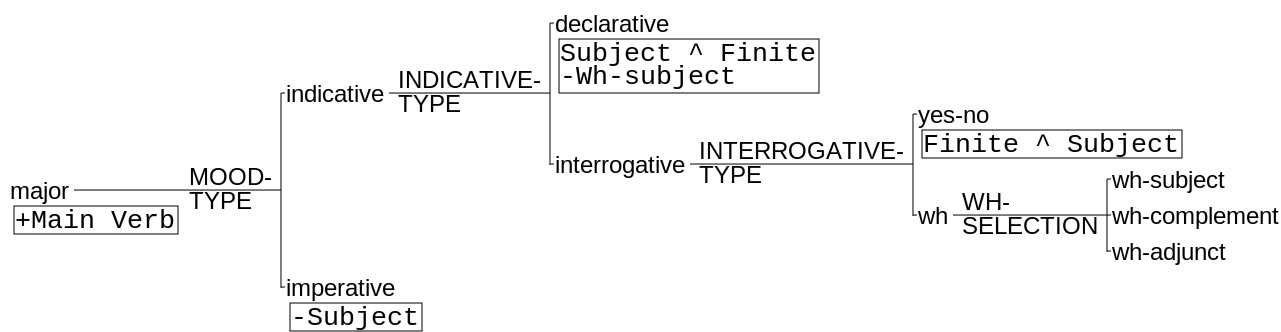
\includegraphics[width=0.91\textwidth]{Figures/Example/just-mood.pdf}      
    \caption{A fragment of mood system from \citet[366]{Halliday2013}}
    \label{fig:just-mood}
\end{figure}

The system network fragment in Figure \ref{fig:just-mood} contains the realisation rules positioned in rectangles below a few features. These realisation rules indicate what shall be reflected in the structure when a feature is selected (discussed already in Section \ref{sec:problem}). The converse is also true: if structure contains a certain pattern then it is a (potential) manifestation of a given feature.

For example the structure of a \textit{major} clause needs to have a predicate or Main Verb element realised. In the parsing process, testing whether there is a unit functioning as Main Verb below in the clause node suffices to assign the \textit{major} feature to that clause. Next, if the clause has no unit functioning as Subject then it shall be assigned \textit{imperative} feature otherwise the \textit{indicative} one. Further the INDICATIVE-TYPE system is enabled. Here the test is whether a Subject node is positioned in front of the Finite node and whether the Subject contain the preposition ``who''. This sort of queries on the structure can be formulated as \textit{structure patterns} (see Section \ref{sec:pattern-graphs}) and associated to features in the system network in the same manner the realisation rules are. 

The pattern recognition plays an essential role in current parsing method for fleshing out the constituent backbone with systemic selections. In the parsing process the structural patterns are tested whether they \textit{match} (see Section \ref{sec:pattern-graph-matching}) anywhere in the constituency structure and if so then the matched nodes are enriched with the features proved in the pattern (described in Section \ref{sec:pattern-based-operations}). 

The structural patterns in this work are expressed as \textit{graph patterns} (described in Section \ref{sec:pattern-graphs}). Note that I employ graph and not tree patterns because the tree patterns are too restrictive for the purpose of the current work. While most of the time they are hierarchically structured as a tree there are few patterns that involve sibling connections or nodes with more than one parent. In both cases the tree structure is broken. The graph approach allows a wide range of structural configurations including the trees. 

The enrichment stage of the parsing process comprises of a series of graph pattern matching operations that in case of success leads to the enrichment of the constituency structure with the features given in the graph pattern. This mechanism is described in detail in the Section \ref{sec:enrichment-stage}. 

In this work most of the graph patterns have been manually created. Because this is laborious exercise only a few system networks have been covered in the implementation of the parser. Nonetheless they suffice for deriving some conclusions regarding the parsing approach. The future work may investigate how can graph patterns be generated automatically from the realisation rules of large grammars such as Nigel grammar. 

The two main system networks targeted in this are MOOD and TRANSITIVITY (both briefly described in Chapter \ref{ch:sfg}). The MOOD network is composed of features which can be identified through graph patterns involving only the unit classes and functions provided in the constituency structure (described in Chapter \ref{ch:parsing-algorithm}). The TRANSITIVITY network requires a lexical-semantic database in order to derive graph patterns. This work employs the Process Type Database (PTDB) \citep{Neale2002} to aid enrichment with TRANSITIVITY features described in Chapter \ref{ch:enrichment-stage}.  



%Moreover if the syntagmatic account is available then they can serve as paradigmatic context (similar to the one available during generation task) for traversing the system network and extend to the full set of systemic features. This sort of description can restrict the search space to applicable network parts and provide to an extent traversal context during analysis task.


%...

%solution to feature enrichment. Transitivity


%The second stage of constituent enrichment by network traversal can be further aided by checking an arbitrary set of patterns for preselecting even more features recoverable via lexico-syntactic patterns. 


%\todo[inline]{I Reuse the structural account from other theories}
%\todo[inline]{
%    Your proposed solution to this problem, and the goal of the thesis,
%    is therefore to add some more structural information to a
%    complete augmented SFG account by drawing on frameworks which
%    have demonstrated coverage of structural detail and which
%    also have supported computational instantiation. This will
%    be shown and evaluated in the thesis.}
%
%\todo[inline]{
%    Reuse structural accounts from other theories that have shown to work well computationally.
%Could use famous Chomskyan approach but will use it latter for a more specific problem, that of finding covert constituents (give example of null subject in embedded clause). Instead I turn to Dependency Grammar that increasingly gained popularity in the last 15 years. It has been shown to be computationally fast and it is compatible in many ways with SFG which I will show latter how (mapping DG to SFG). }
%
%\todo[inline]{how: (1) by aligning the primitives and drawing cross-theoretical bridges (see section X), (2) then by mapping grammars (see section Y), (3) implemented using graph transformations (see section Z)}
%
%\todo[inline]{II Enrich the constituency structure with features (since the original goal is to have rich language analysis), that in traditional sense are spanning from purely syntactic (such as tense, voice, case, gender, number etc.) or more semantic or even pragmatic (such as semantic role labels, speech acts, sentiment and appraisal and others) }
%
%\todo[inline]{how: (1) by mapping structure to features (SFL Mood) (see section X), (2) by mapping lexical-semantic resources to fragments of syntactic structure and lexis (lexis contextualised by syntactic structure) (SFL Transitivity) (see section Y), (3) implemented by graph pattern matching (see section Z)}
%
%\todo[inline]{
%    So, the thesis goal and outline will be to (and you list them
%    explicitly like this too):\newline
%    - characterise SFL in its two major variants\newline
%    - characterise the previous attempts to parse with SFL and their problems\newline
%    - set out two further linguistic frameworks which (a) have\newline
%    strong accounts of structural relationships, (b) have shown
%    themselves supportive of computational instantiation, and (c) can
%    be shown to exhibit suggestive theoretical/descriptive
%    links with SFG: in particular, DG and GB.
%    
%    Chapter X does this for DG
%    Chapter Y does this for GB.}

\subsection{Parsimonious Vole architecture}
\label{sec:architecture}
The current thesis is accompanied by a software implementation - the Parsimonious Vole parser. It is written in Python programming language and is available as open source distribution\footnote{\url{https://bitbucket.org/lps/parsimonious-vole}} . This section provides an overview to the construction process.

The parser follows a pipeline architecture depicted in Figure \ref{fig:pipeline-overview} where, starting from an input text, a rich systemic functional constituency structure is progressively built. Figure \ref{fig:pipeline-overview} provides three types of boxes: the rounded rectangles represent the parsing steps, the green trapezoid boxes represent input and output data while the orange double framed trapezoid boxes represent additional resources involved in the parsing step. The parsing steps linearly flow from one to the next via green trapezoid boxes on the left-hand side, which represent input-output data in between the steps. On the right-hand side are positioned double edged orange trapezoids representing fixed resources needed by some operations. For example, the \textit{constituency graph creation} step takes a normalised dependency graph for input and produces a constituency graph as output.

On the right-hand side a series of green vertical arrows are provided naming phases in parsing process (spanning one ore more process steps) where the first one, \textit{Graph Building} (spanning the first three process steps), accomplish construction of the constituency backbone (corresponding to the syntagmatic account described in Section \ref{sec:syntagmatic-account} above) and the second phase \textit{Graph Enrichment} (spanning the last three process steps) flashes out the backbone with features (described in Section \ref{sec:paradigmatic-account}). 

\begin{figure}[!ht]
    \begin{tikzpicture}[node distance=1.2em, scale=0.85, transform shape]
    % aLVL 0
    \node[](data) {}; % invisible node
    \node[right=12em of data](process) {}; % invisible node
    \node[right=12em of process](resource) {}; % invisible node 
    \node[right=9.5em of resource](flow) {}; % invisible node 
    
    % aLVL 1
    \node[data,anchor=center, below=-2em of data] (text) {Input Text};
    \node[task,anchor=center, below=-2em of process] (dep-parse) { Dependecy Parsing};
    \draw[sequence,->] (text) -- (dep-parse);
    
    % aLVL 2
    \node[data,anchor=center, below=6.5em of data] (dep-graph) {Dependecy Graph};
    \node[task,anchor=center, below=6em of process] (correction) {Error Correction \& \\ Graph Normalization};
    \draw[sequence,->] (dep-graph) -- (correction);
    \draw[sequence,->] (dep-parse.south) -- ++(0,-1.5em)  -| (dep-graph.north);
    
    % resources
    \node[persistent-data,anchor=center, below=4em of resource] (error-graph) {Common Error \\ Graph Patterns};
    \node[persistent-data,anchor=center, below=8em of resource] (norm-graph) {Normalization \\ Graph Patterns};
    
    \draw[sequence,->] (error-graph.west) -- ++(-1.5em,0)  |- (correction.east);
    \draw[sequence,->] (norm-graph.west) -- ++(-1.5em,0)  |- (correction.east);
    
    % aLVL 3
    \node[data,anchor=center, below=14em of data] (norm-dep-graph) {Normalised \\ Dependency Graph };
    \node[task,anchor=center, below=14em of process] (const-cr) {Constituency Graph \\ Creation};
    \draw[sequence,->] (norm-dep-graph) -- (const-cr);
    \draw[sequence,->] (correction.south) -- ++(0,-1.5em)  -| (norm-dep-graph.north);
    
    % resources
    \node[persistent-data,anchor=center, below=14.22em of resource] (rule-table) {Rule Table}; % 12.425
    \draw[sequence,->] (rule-table.west) --  (const-cr.east);
    
    % aLVL 4
    \node[data,anchor=center, below=24em of data] (const-gr) {Constituency Graph };
    \node[task,anchor=center, below=23.5em of process] (const-gr-enr) {Mood\\Enrichment};
    \draw[sequence,->] (const-gr) -- (const-gr-enr);
    \draw[sequence,->] (const-cr.south) -- ++(0,-1.5em)  -| (const-gr.north);
    
    %resources
    \node[persistent-data,anchor=center, below=21em of resource] (sys-net) {System Network};
    \node[persistent-data,anchor=center, below=23.5em of resource] (feat-dict) {Feature-rich \\ Dictionaries};
    \node[persistent-data,anchor=center, below=27em of resource] (sys-feat-gm) {Mood \\ Graph Patterns};
    \draw[sequence,->] (feat-dict.west) --  (const-gr-enr.east);
    \draw[sequence,->] (sys-net.west) -- ++(-.79em,0)  |- (const-gr-enr.east);
    \draw[sequence,->] (sys-feat-gm.west) -- ++(-1.9em,0)  |- (const-gr-enr.east);
    
    % aLVL 5
    \node[data,anchor=center, below=31.5em of data] (enriched-gr) {(Feature Enriched) \\ Constituency Graph };
    \node[task,anchor=center, below=31.5em of process] (null-cr) {Null Element \\ Creation};
    \draw[sequence,->] (enriched-gr) -- (null-cr);
    \draw[sequence,->] (const-gr-enr.south) -- ++(0,-1.5em)  -| (enriched-gr.north);
    
    %resources
    \node[persistent-data,anchor=center, below=31.5em of resource] (null-gr) {Null Element \\ Graph Patterns};
    \draw[sequence,->] (null-gr) -- (null-cr);
    
    %aLVL 6
    \node[data,anchor=center, below=38.5em of data] (null-enr-gr) {(Null Enriched) \\ Constituency Graph };
    \node[task,anchor=center, below=38.5em of process] (sem-enr) {Transitivity \\ Enrichment};
    \draw[sequence,->] (null-enr-gr) -- (sem-enr);
    \draw[sequence,->] (null-cr.south) -- ++(0,-1.5em)  -| (null-enr-gr.north);
    
    %resources 
    \node[persistent-data,anchor=center, below=36em of resource] (sys-net1) {System Network};
    \node[persistent-data,anchor=center, below=38.5em of resource] (ptdb) {Process Type \\ Database};
    \node[persistent-data,anchor=center, below=42em of resource] (pc-gp) {Transitivity \\ Graph Patterns};
    \draw[sequence,->] (sys-net1.west) -- ++(-1.35em,0)  |- (sem-enr.east);
    \draw[sequence,->] (pc-gp.west) -- ++(-2.4em,0)  |- (sem-enr.east);
    \draw[sequence,->] (ptdb.west) -- (sem-enr.east);
    
    %aLVL 7
    
    \node[data,anchor=center, below=45em of data] (final) {Rich Constituency Graph};
    \draw[sequence,->] (sem-enr.south) -- ++(0,-1.5em)  -| (final.north);
    
    % vertical arrows
    
%    \node[flow-arrow, below=-2em of flow] (bootstrapping) {Bootstrapping};
%    \node[flow-arrow, below=7em of flow] (pre-processing) {Pre-processing};
%    \node[flow-arrow, below=15em of flow] (creation) {Graph \\ Building};
    \node[flow-arrow, below=7em of flow, minimum width=22em] (building) {Graph Building};
    \node[flow-arrow, below=32.5em of flow, minimum width=26em] (enrichment) {(Increasingly Semantic) Graph Enrichment};
    \end{tikzpicture}
    \caption[]{The parsing process pipeline}
    \label{fig:pipeline-overview}
\end{figure}

One important feature of this implementation is its heavy reliance on graph pattern matching and other operations using graph patterns described in Chapter \ref{ch:data-structures}. 

The parsing process starts with an input English text and ends with production of a Rich Constituency Graph. Input Text is first parsed with the Stanford Dependency parser \citep{chen2014fast} version 3.5\footnote{\url{https://nlp.stanford.edu/software/nndep.html}} producing a Dependency Graph.

The dependency graphs often contain errors. Some of these errors are predictable and so easy to identify and correct. Also, some linguistic phenomena are treated in a slightly different manner than that proposed in the current thesis. Therefore the dependency graph produced by the Stanford parser is \textit{Corrected and Normalised} using graph pattern matching against collections of known errors and a set of normalization rules encoded as graph patterns.

Once normalised the dependency graph is ready to guide the \textit{building process} of the systemic functional constituency graph. Through a traversal of the dependency graph the constituency graph is parallelly constructed guided by a mapping \textit{Rule Table}. The mappings indicate what operation to perform on the newly emerging graph given the visited dependency node and its incoming and outgoing relations. Even if it a distinct structure, the constituency graph is, in a way, a transformation of the dependency graph. It constitutes the syntactic backbone on which the subsequent enrichment phases are performed.

Next follows the phase where each constituent node of the syntactic backbone is \textit{enriched} with features, some of which are of a \textit{syntactic} and others of a \textit{semantic} nature. In between these enrichment phases there is an additional construction process adding where needed \textit{empty constituents} that play an important role in semantic enrichment. The enrichment steps use additional resources such as \textit{system networks}, \textit{feature rich lexicons}, \textit{graph patterns} and a \textit{semantic database}. The \textit{null element creation} process also needs a collection of graph patterns for identifying where and what kind of null elements occur as motivated in Section \ref{sec:problem} and explained in detail in Chapter \ref{ch:gbt}. The final result of the process is a \textit{Rich Constituency Graph} of the original text comprising a substantial set of systemic feature selections associated with constituting units of structure. 

The the detailed parser implementation choices and developed algorithms are presented in Chapters \ref{ch:parsing-algorithm} and \ref{ch:enrichment-stage}.

\subsection{Research questions and contributions} % In a nutshell 
This thesis addresses the following questions:
\begin{itemize}
%    \item What is a computationally feasible method to parse with systemic functional grammars using a syntactic backbone?
    \item To what extent techniques from other areas of computational linguistics can be reused for the SFL parsing? 
    \item To what degree the syntactic structures of the Dependency Grammar and Systemic Functional Grammar are compatible to undergo a transformation from one into the other?
    \item Is Stanford dependency grammar suitable as a syntactic backbone for Systemic Functional Grammar parsing?
%     along with an implemented method to transform from one structure to another.
    
%    \item If so
    %	\item what degree of delicacy in paradigmatic choices can be provided from the systemic networks of SF grammars?
    %	\item How to approach semantic parsing with SFGs provided the PTDB resource?
    %	\item How to approach Transitivity parsing with Process Type Database and how suitable it is for the task?
    \item Can the Process Type Database be used as a resource for SFG Transitivity parsing?
    \item How can Government and Binding Theory be used for detecting places of null elements in the context of SFL constituency structure?
%    of external predicates in the context of SFG Transitivity parsing with PTDB?
    
\end{itemize}

Also it brings the following theoretical and practical contributions:
\begin{itemize}

%    \item A fast engine for graph pattern matching which can also update and insert new nodes.
    \item A set of theoretical principles and generalizations establishing cross-theory links between Dependency Grammar and SFL. 
%    \item A set of theoretical principles and generalizations establishing cross-theory links between Dependency Grammar and SFL. 
    \item A set of mapping rules between Stanford Dependency v3.5 to SFG constituency structure.
    \item A parallel graph construction process for creating SF syntactic backbone.
    
    \item A flexible and expressive method to represent systemic features as graph patterns and a strategy for choice propagation in the systemic networks.
    \item A set of pattern graphs covering Mood, Transitivity and a few other small system networks.
    \item A clean machine readable version of the PTDB. 
    \item A method to transform PTDB into Transitivity graph patterns. 

    \item Several principles for detecting null elements in the sentence which were translated from the Government and Binding Theory (GBT) into Dependency and SFL terms. 
    \item Implementation of the translated GBT principles as graph patterns corresponding usable to identify the null elements in a sentence.
%    and represented them as graph patterns used  These generalizations serve for semantic parsing where is very helpful to identify the external arguments of verbs.
    \item A small test corpus to evaluate the Parsimonious Vole parser.
\end{itemize}

\section{Overview of the thesis}
\label{sec:thesis-structure}

Chapter \ref{ch:introduction} has provided an introductions to the work described in this thesis. It has indicated the are to which it seeks to contribute, and described the motivation of work from an applied and a theoretical perspective. In Chapter \ref{ch:sota} a list of selected works on parsing with SFG is presented and briefly discussed. 

Chapter \ref{ch:sfg} provides and overview of the SFL theoretical foundations. There are two outstanding traditions in SFL each providing a theory of grammar. First is developed in Sydney by Halliday, Matthiessen, Hassan, Martin, Rose and others. The second is developed in Cardiff by Fawcett, Tucker, Tench and others. I present both schools in first two sections of the chapter and then, in the third section, I provide a comparative critical discussion on both theories of grammar motivating relaxation of the rank scale, approach to structure formation, unit classes and few other concepts relevant to current work. 

In the following chapter I provide a description of the grammar implemented in the Parsimonious Vole which. It is a selection of unit classes from both Sydney and Cardiff Grammars following the theoretical motivation from the previous chapter. Here is also presented a selection of two system networks: MOOD and TRANSITIVITY that were selected to demonstrate how the current parsing method works. The former system network is tightly linked to the syntagmatic variations in the structure whereas the latter describes ideational choices of the semantic structures and, thus, is farther from the surface variations. In order to integrate this system network I use a lexical database of verb meanings called Process Type Database \citet{Neale2002}. 


Chapter \ref{ch:dependecy-grammar} introduces the Dependency Grammar \citeyear{Tesniere59}, starting with it's origins and foundations, evolution into its modern form, its applications in computational contexts particularly highlighting the Stanford grammatical model and parser. The usage of dependency grammar and dependency parse graphs is motivated in \ref{sec:syntagmatic-account} as the primary input into the current parsing pipeline for creating the constituency structure. The last part of the chapter provides a cross theoretical bridge from the dependency grammar towards the systemic functional grammar integrated into the Parsimonious Vole implementation. 

Next chapter starts with an introduction of Government and Binding Theory (GBT) explaining where the empty constituents occur in sentences. These constituents were motivated in \ref{sec:problem} and are a part of solution for parsing with TRANSITIVITY system network. The second section of the chapter provides an inventory of different null elements and the last section provides, just like in the previous chapter, a cross theoretical overview, this time from GBT phrase parse structures into Stanford dependency grammar.

Chapter \ref{ch:data-structures} provides the building blocs of the algorithms of this thesis. It makes the transition from the linguistic theoretic presentations towards the computer science foundations introducing necessary typed sets, feature structures and graphs. These concepts are employed in the chapters that follow to represent linguistic constructs described in the previous chapters. An important role, in the current work, play the pattern graphs and the operations enabled by using them presented in Sections \ref{sec:pattern-graphs} -- \ref{sec:pattern-based-operations}. The system networks, are defined in a simplified form corresponding to how they are currently used followed by a brief discussion.

The first phase of the parsing pipeline (see Figure \ref{fig:pipeline-overview}) concerning the constituency graph building is entirely covered by the Chapter \ref{ch:parsing-algorithm}. It presents how the input dependency graphs are first corrected and normalised and the how they are rewritten, using a custom algorithm, into constituency graphs. 

The second phase of the pipeline (see Figure \ref{fig:pipeline-overview}) concerning the enrichment of the  constituency graph with increasingly more semantic features is described in the Chapter \ref{ch:enrichment-stage}. It addresses two main system networks, that of MOOD and TRANSITIVITY introduced in Chapter \ref{ch:the-grammar}. The MOOD features are close to syntactic variation of text and can be addressed via graph patterns alone in the first part of the chapter. The TRANSITIVITY features are semantic in nature and require additional lexical-semantic resources from which graph patterns are generated first and then applied to enrich the constituency graph.

Chapter \ref{ch:evaluation} describes how the Parsimonious Vole parser was evaluated with a small evaluation set created for this parser. The chapter describes the evaluation settings and the results for syntactic and semantic parsing. Chapter \ref{ch:conclusions} concludes this work by providing a thesis summary overview, indications for practical applications of this work and future directions to follow. 


%\todo[inline]{
%    1: introduction \\
%    2: SFG parsing problem (simple explanation) and SOTA \\
%    3: Architecture presentation, introducing challenges of every step and make future references, also the structure of the thesis. \\
%    4: SFL grammar \\
%    5: Dep Grammar \\
%    5: GBT (has to stay here somehow) \\
%%    6: the data structures + operations \\ no more data structures, dictribute where needed
%    7: the structure creation (introducing basic computer scientific definitions of data structures and other needs) (introducing the exact SFG grammar constituents) \\
%    8: the syntactic feature enrichment (introducing basic computer scientific definitions of data structures and other needs) (introducing exact Mood features) \\
%
%    9: the semantic feature enrichment (introducing basic computer scientific definitions of data structures and other needs) (introducing exact Cardiff Transitivity features) \\
%
%
%    10: Empirical Evaluation \\
%    11: Conclusions (what has been achieved and outlook) \\   
%}